%!TEX root = ../main.tex
%%%%%%%%%%%%%%%%%%%%%%%%%%%%%%%%%%
% Links:
%
% Difficulty: Easy/Medium Companies: 
%%%%%%%%%%%%%%%%%%%%%%%%%%%%%%%%%%

%\chapterimage{header}

\chapter{Power set generation}
\label{ch:power_set}
\section*{Introduction}
The concept of power set is familiar to many because it is introduced very early during
introductionary math courses on set theory. The problem described in this chapter is about writing
an algorithm that is capable of finding the powerset of a given set. Two main solution approach are
presented here, one that is strightforward deriving immediately from the recursive definition of
power set\footnote{The following is the recursive definition of powerset. In words the powerset of an empty
set is a set contains as only element the empty set itself. For a non-empty set, let $e$ be an
element of the set and T be the original set minus $e$ (relative complement). The powerset can
be then definied as the union of two distinct powersets. The powerset of T (all the subsets not
containing $e$) and the powerset of T modified in a way such that $e$ is added to all of its
element.
\begin{equation}
	\mathcal{P}(S)=\begin{cases} 
\{\{\}\} & \text{if } P=\{\} \\
P\{T\} \bigcup \{t \in P\{T\} : t \cup \{e\}\} \text{ where } e \in P, \text{ and } T = P \setminus \{e\} & \text{otherwise}
\end{cases}
\label{eq:power_set_recursive_definition}
\end{equation} 
} (See Equation \ref{eq:power_set_recursive_definition}), while the other is based on a clever
observation about the distribution of the bits among the integers from $0$ to the size of the
powerset. The problem is usually presented in a very direct manner with a short and concise
statement because the interviewer is expecting the candidate to be already familiar with the
concept.



\section{Problem statement}
	\begin{exercise}
		Write a function that given a set of elements $P$ returns its power-set. A power-set of a set $P$,
		(here denoted as $\mathcal{P}(S)$ is the set of all its subsets including the empty subset
		$\emptyset$ and $P$ itself.

		\begin{example}
			\hfill \\
			For example, given the set $P=\{a,b,c\}$, the following two sets are both correct outputs for
			this problem:
			\begin{equation*}
				\{\{\}, \{b,c\}, \{a\}, \{a,b\}, \{a,b,c\}, \{b\}, \{a,c\}, \{c\} \}
			\end{equation*}
			\begin{equation*}
				\{\{\}, \{a\}, \{b\}, \{c\}, \{a,b\}, \{b,c\}, \{a,c\}, \{a,b,c\} \}
			\end{equation*}
			
		\end{example}
	\end{exercise}
\section{Clarification Questions}

\begin{QandA}
	\item What is the maximum size of the input?
	\begin{answered}
		\textit{The maximum number of element is strictly less than $n < 32$.}
	\end{answered}
	
	\item Are all the element in the collection distinct?
	\begin{answered}
		\textit{No, the elements are not necessarily distinct. $S$ can contain duplicates.}
	\end{answered}

	\item Can the subset in the power-set appear in any order?
	\begin{answered}
		\textit{Yes, subsets can appear in any order.}
	\end{answered}
\end{QandA}

\section{Discussion}
There is one key point that should immediately be noticed: \textbf{The powerset of a collection of
	$n$ elements has size} $\boxed{2^n}$\footnote{The proof of this fact is relatively easy and it boils
	down to the fact that a subset of $P$ is basically $P$ with possibly some of the elements
	removed from it. Because we two possible choices we can make for every element of $S$ (either
	remove or not remove and element) then the total number of possible subset is: $2 \times 2
	\times \ldots \times 2 = 2^{|P|}$. Two choices for the first element, two for the second, and so
	on until the last element of $P$.} . This fact should be immediately pointed out during the
	interview, stressing the fact that the constraint $n < 32$ is a strong hint towards the fact
	that an exponential solution is expected. After-all we are required to output all the elements
	of the powerset, and thus the complexity of any algorithm solving this problem cannot be less
	than the size of the powerset itself. Doing so shows general knowledge on set theory and the
	ability to link and use that knowledge with the problem statement.


\subsection{Backtracking}
The first solution presented in this chapter is based on the fact that that during the generation of
one of the elements of the power-set a decision has to be taken for each element of the original
set, on whether to include the element or not into the subset. When a decision for the first element
is taken then what we are left with is $|P|-1$ decisions before we have created a valid subset of
$|P|$. 
This kind of process can be easily visualized with a tree where a node at level $i$
represents a decision for the $i^{th}$ element and a path from the root to a leaf uniquely
identifies a subset of $P$ i.e. $n$ decisions. 
All paths from the root to the leafs thus, represent the power set. In
order to solve this problem we have to explore the entirety of this tree. An example of such tree is
shown in Figure \ref{ref:power_set_decision_trees}.

One general way to deal with such type of problems is by using backtracking to try all possible
decision paths for each of the elements. The general idea is that we are going to, for all elements
starting from the first until the last, to explore the two possibilities: take or exclude the
element from the subset. Backtracking is a general algorithm that allows to enumerate and explore
large search spaces like this one. The main idea is that we first try to stick with a decision for
the first element, and we continue from there to generate all possible subsets where said decision
is never changed. When there is no more subset to generate, we backtrack and change our first
decisions to the next possible one and repeat the process of generating all possible subsets.
The proposed solution will incrementally construct one subset at the time, using an integer variable
to keep track of which element we are currently
deciding to include or exclude. The base case of the recursion happen when there is no more decision
to take, meaning that the current subset is ready to be included in the solution (it has been
produced after $n$ decision steps).

The C++ code implementing the idea above is shown in Listing \ref{list:power_set_backtracking}. The
complexity of this solution is exponential i.e. $O(2^n)$ which as already pointed out is as good as
it gets.

\begin{minipage}{\linewidth}
	\lstinputlisting[language=c++, caption="C++ to the power set generation using backtracking",label=list:power_set_backtracking]{sources/power_set/power_set_backtracking.cpp}
\end{minipage}

\begin{figure}
	\centering
	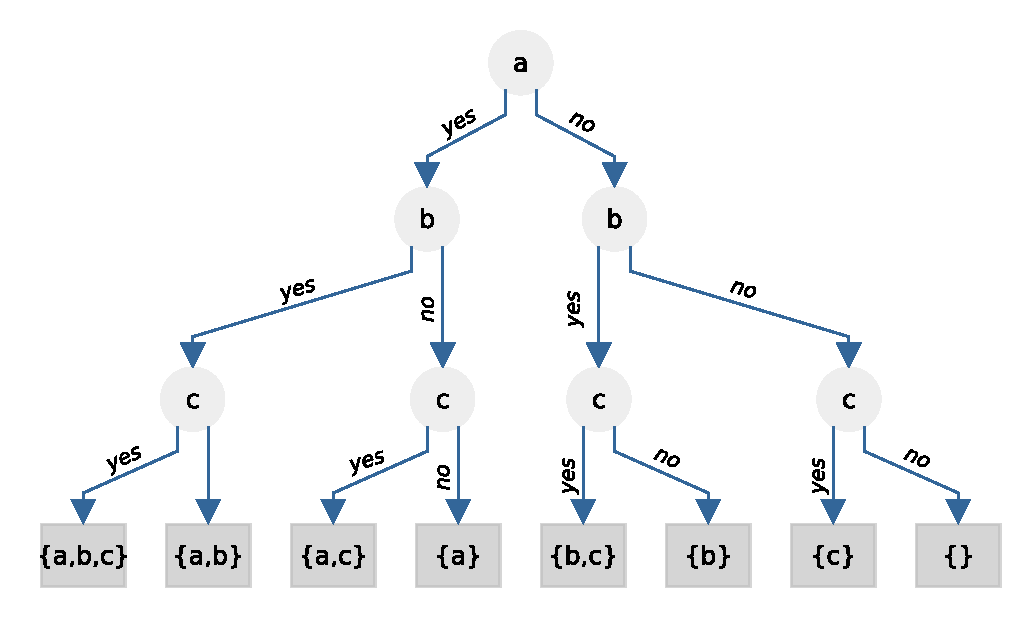
\includegraphics[width=\textwidth]{sources/power_set/images/tree}
	\caption[Decision tree for the power-set generation using backtracking.]{Decision tree for the power-set generation using backtracking. At level $i$ are the decision for the element $i$ in the original set. A labal marked with yes identifies the decision to take the corrensponding element into the subset, while a node labeled with no the opposite. At the last level is the powerset.}
	\label{ref:power_set_decision_trees}
\end{figure}

The advantages of using the backtracking framework to solve this problem is that, once we notice
that this problem can be solved by fully exploring the search tree, then we can immediately
start writing the code and rely on our experience as backtracking algorithm writers to implement a correct
solution with the added bonuses of being concise and short when written in a recusive form  as well
as well understood.
The downside is that the iterative implementation can be a little harder and more verbose to write.
Regardless of which one you choose, the interviewer is going to be pleased with your code provided you get to the final solution
without making too many implementation mistakes (forgetting to add the base case, or coding it wrong
is a pretty common one).

\subsection{Bit Manipulation}
Another approach that can be used to solve this problem is based on the fact that the values of the
bits of the numbers $\{0,1,2,\ldots, s^n-1\}$  already provide all the information necessary to make
the decision weather to include or not an element from the original set. 
The main idea is that the binary representation of the numbers from $0$ to $2^{n}-1$ is basically
the powerset of $n$ bits.
In other words, the binary representation of any of those numbers can be used to build one subset out
of the $n$ elements of the input set. 
For instance given the input $S=\{a,b,c\}$ the Table \ref{tab:mapping_value_bits} shows numbers from $0$ to $2^3-1 = 8$ and their bit
representation (second column) and how such information about which bit is set or not can be used to construct one
subset of the power-set of $P$ (third column). When the $i^{th}$ bit is set i.e. its value it $1$, it means that
corresponding $i^{th}$ element of $P$ is taken, while a non-set bit (with value $0$) means it is
excluded.

\begin{table}
	\centering
	\begin{tabular}{|l|l|l|}
		\hline
		Value & Bits & Subset\\ \hline
		0     & 000  & $\{\}$\\ \hline
		1     & 001  & $\{c\}$\\ \hline
		2     & 010  & $\{b\}$\\ \hline
		3     & 011  & $\{b,c\}$\\ \hline
		4     & 100  & $\{a\}$\\ \hline
		5     & 101  & $\{a,c\}$\\ \hline
		6     & 110  & $\{a,b\}$\\ \hline
		7     & 111  & $\{a,b,c\}$ \\ \hline
	\end{tabular}
	\caption[Mapping between bits and element of the powerset.]{This table shows a 1-to-1 mapping between integer values, their binary representation and an element of the powerset.}
	\label{tab:mapping_value_bits}
\end{table}

This idea can be used to write an algorithm in which all the numbers in the range $\{0,1,2,\ldots,
s^n-1\}$ are considered and each of them is used to generate a subset of the final solution.
Basically every number from such range maps uniquely to a subset of the powerset. It is really not
surprising when we think about the meaning of a bit in the binary representation of integers. One
can build a number by summing up powers of $2$ and the bits contains the information on whether a
certain power of two should be added to the final value for the represented number or not. With $n$
bits one can represents $2^n$ numbers, each corrensponding to one subset of the powerset of those
$n$ bits.

Listing \ref{list:power_set_bits} shows  a possible C++ implementation of the idea above\footnote{Notice the usage of the \texttt{reserve}
function that should be used in all those scenario when we already know the final size of the
collection we are building. This saves times because avoids intermediate allocation and copy that
must happen during the resize of the vector.}. The complexity of this implementation is, not
surprisingly, $O(2^n)$\footnote{Not considering the constant price of $32$ that we pay for each
subset generation due to the fact that we need to inspect the value of all of the bits}. Also please
pay attention to the fact that the proposed implementation assumes that the size of
\lstinline[columns=fixed]{int} is $4$ bytes, which is true for most architecture but not for all\cite{cit::std::fundamentaltypes}. A better
implementation would use \lstinline[columns=fixed]{std::numeric_limits<int>::digits} instead of
the magic number $32$.


\begin{minipage}{\linewidth}
	\lstinputlisting[language=c++, caption="C++ backtracking solution to the problem of generating the powerset.",label=list:power_set_bits]{sources/power_set/power_set_bit_manipulation.cpp}
\end{minipage}

%\section{Common variations}

%\section{Conclusion}
